\chapter{Implementacija i korisničko sučelje}
		
		
		\section{Korištene tehnologije i alati}
		
			\textbf{\textit{dio 2. revizije}}
			
			 \textit{Detaljno navesti sve tehnologije i alate koji su primijenjeni pri izradi dokumentacije i aplikacije. Ukratko ih opisati, te navesti njihovo značenje i mjesto primjene. Za svaki navedeni alat i tehnologiju je potrebno \textbf{navesti internet poveznicu} gdje se mogu preuzeti ili više saznati o njima}.
			
			
			\eject 
		
	
		\section{Ispitivanje programskog rješenja}
			
			
			\subsection{Ispitivanje komponenti}
			Testirali smo 8 ispitnih slučajeva unoseći ispravne i neispravne podatke te provjeravajući vraća li sustav odgovore kakve očekujemo. Od osam ispitnih primjera, četiri se odnose na šetače te četiri na udruge. Rezultati i opisi pojedinih testova su priloženi ispod. Kao što ćemo vidjeti u rezultatima, svi su ispiti prolazni jer smo pri upisu neispravnih podataka i očekivali odgovore različite od 200 OK.
			
			\subsubsection{1. ispitni primjer - registracija udruge sa zauzetim OIB-om}
			
			U ispitnom primjeru prvo smo stvorili i registrirali prvu udrugu sa zadanim OIB-om 22000000000. Dobili smo očekivani odgovor sa statusom 200 OK. Zatim smo pokušali registrirati drugu udrugu sa istim tim OIB-om (ali drugačijim korisničkim imenom, koji također mora biti jedinstven). Dobili smo očekivani odgovor sa statusom 406 NOT ACCEPTABLE. Nakon toga smo promijenili OIB u 22000000001 te ponovno poslali zahtjev za registracijom. Dobili smo očekivani odgovor 200 OK.
			\begin{figure}[H]
				\centerline{
					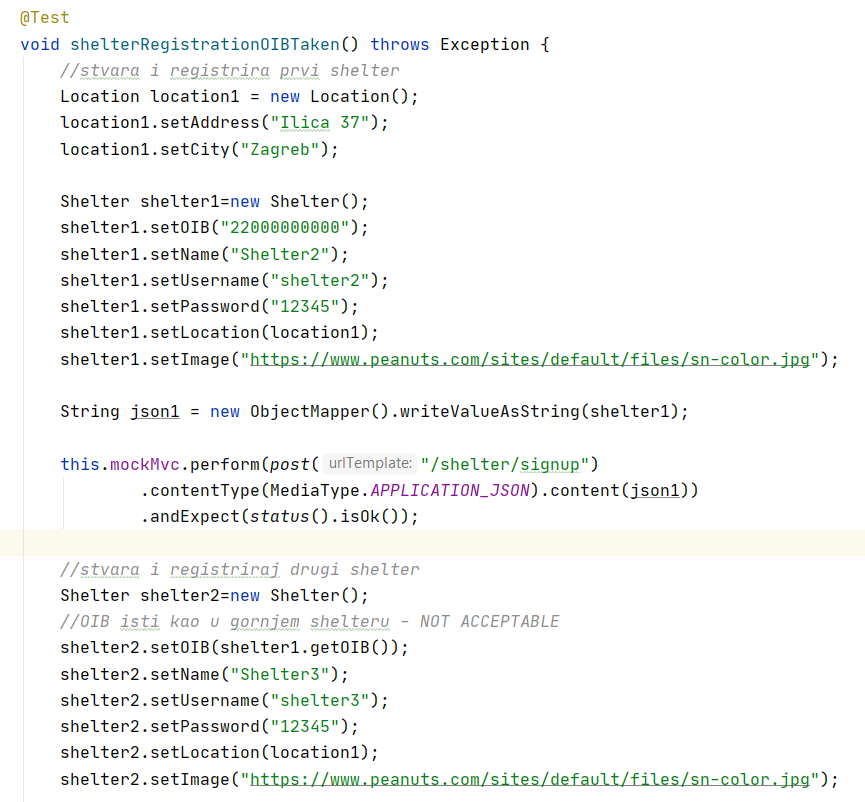
\includegraphics[scale=0.73]{slike/shelter1.1.PNG}}
				\hspace*{-0.21in}
				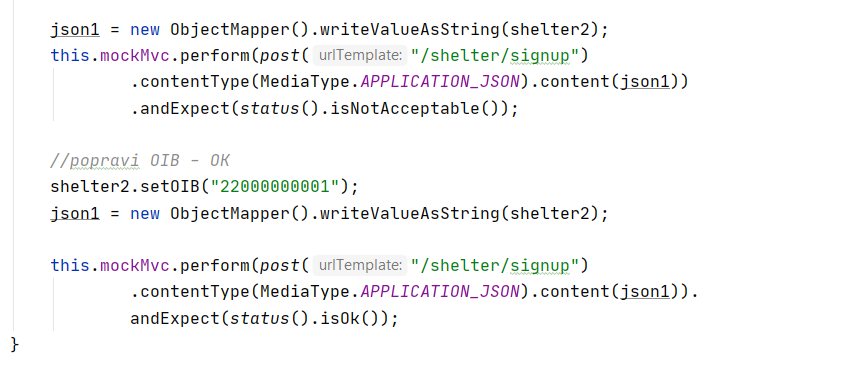
\includegraphics[scale=0.73]{slike/shelter1.2.PNG}
				%veličina slike u odnosu na originalnu datoteku i pozicija slike
				\centering
			\end{figure}
			
			
			
			\subsubsection{2. ispitni primjer - registracija udruge sa zauzetim korisničkim imenom}
			
			U ispitnom primjeru prvo smo stvorili i registrirali prvu udrugu sa zadanim korisničkim imenom "ella". Dobili smo očekivani odgovor sa statusom 200 OK. Zatim smo pokušali registrirati drugu udrugu sa istim tim korisničkim imenom (ali drugačijim OIB-om, koji također mora biti jedinstven). Dobili smo očekivani odgovor sa statusom 409 CONFLICT. Možemo primjetiti da je to drugačiji odgovor od onog u gornjem testu kada šaljemo OIB koji nije jedinstven (409 NOT ACCEPTED). To je zato što smo pomoću tih odgovora razlikovali kakav odgovor tj. feedback treba dati korisniku pri registraciji. Nakon toga smo promijenili korisničko ime u "lily" te ponovno poslali zahtjev za registracijom. Dobili smo očekivani odgovor 200 OK.
			
			\begin{figure}[H]
				\centerline{
					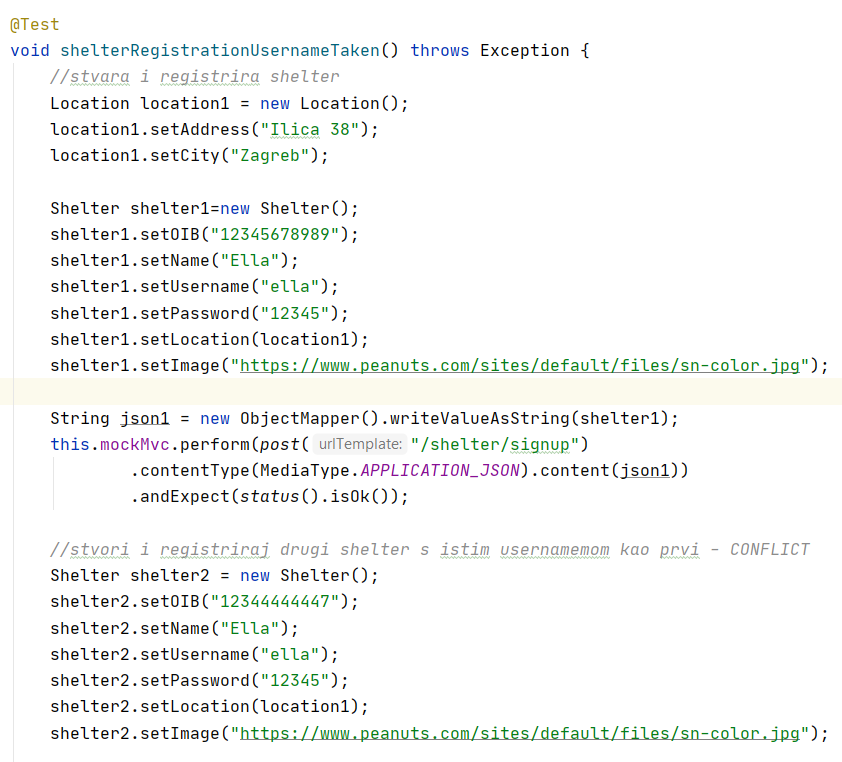
\includegraphics[scale=0.75]{slike/shelter2.1.PNG}}
				\hspace*{-0.22in}
				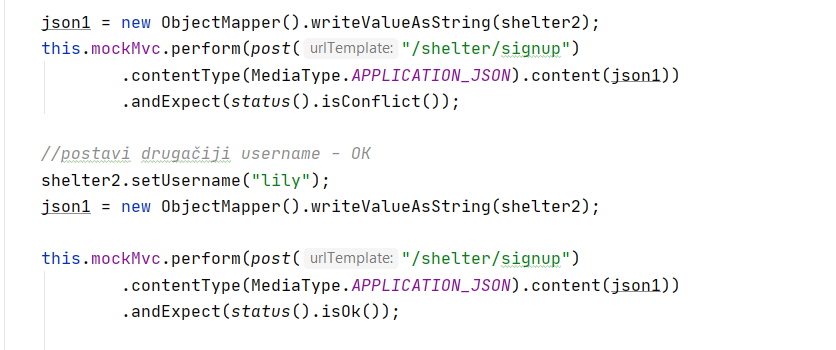
\includegraphics[scale=0.75]{slike/shelter2.2.PNG} %veličina slike u odnosu na originalnu datoteku i pozicija slike
				\centering
			\end{figure}
			
			
			
			\subsubsection{3. ispitni primjer - mijenjanje podataka udruge sa i bez autorizacije }
			
			U ispitnom primjeru prvo smo stvorili i registrirali  udrugu. Dobili smo očekivani odgovor sa statusom 200 OK. Također, u tijelu odgovora nam je vraćena ta udruga koju smo upravo registrirali uz dodatak ID-a udruge koji je stvoren na backendu. Taj vraćeni objekt smo spremili u našu varijablu udruge jer ćemo koristiti vraćeni ID u putanji za mijenjanje podataka. Zatim smo promijenili ime udruge u "NovoIme" te poslali zahtjev za promjenom. Dobili smo očekivani odgovor sa statusom 401 UNAUTHORIZED jer nismo dodali autorizaciju na zahtjev. Nakon toga smo pokušali ponovno sa dodanom autorizacijom te dobili očekivani odgovor 200 OK te udrugu sa promijenjenim imenom u tijelu odgovora. Na kraju smo provjerili da je u vraćenoj udruzi stvarno promijenjeno ime.
			
			\begin{figure}[H]
				\hspace*{-0.5in}
				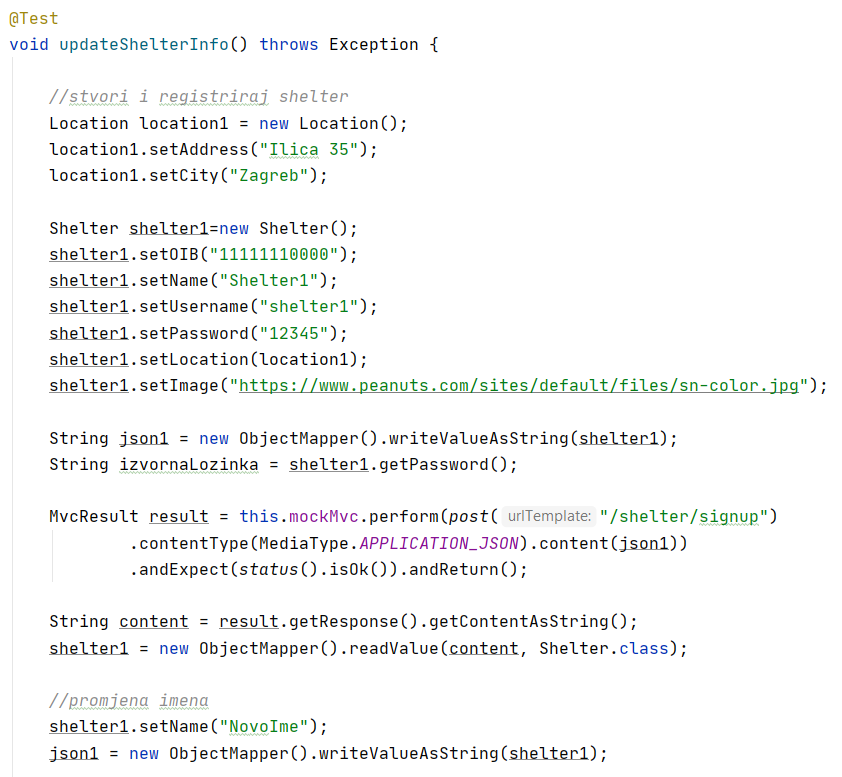
\includegraphics[scale=0.73]{slike/shelter3.1.PNG}
				\hspace*{-0.45in}	
				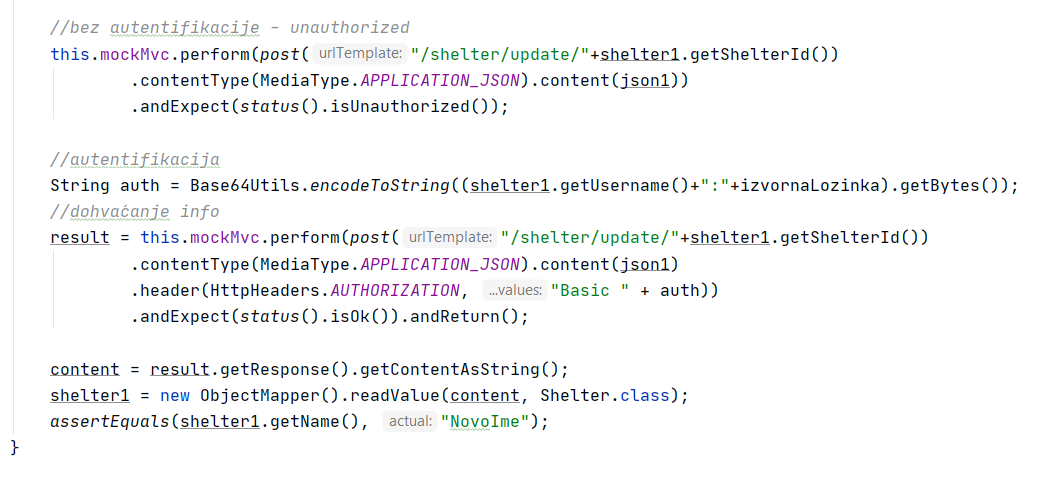
\includegraphics[scale=0.73]{slike/shelter3.2.PNG} %veličina slike u odnosu na originalnu datoteku i pozicija slike
				\centering
			\end{figure}
			
			
			\subsubsection{4. ispitni primjer - brisanje udruge sa i bez autorizacije }
			
			U ispitnom primjeru prvo smo stvorili i registrirali  udrugu. Dobili smo očekivani odgovor sa statusom 200 OK. Također, u tijelu odgovora nam je vraćena ta udruga koju smo upravo registrirali uz dodatak ID-a udruge koji je stvoren na backendu. Taj vraćeni objekt smo spremili u našu varijablu udruge jer ćemo koristiti vraćeni ID u putanji za brisanje udruge. Zatim smo poslali zahtjev za brisanjem bez autorizacije. Dobili smo očekivani odgovor sa statusom 401 UNAUTHORIZED jer nismo dodali autorizaciju na zahtjev. Nakon toga smo pokušali ponovno sa dodanom autorizacijom te dobili očekivani odgovor 200 OK.
			
			\begin{figure}[H]
				\hspace*{-0.93in}
				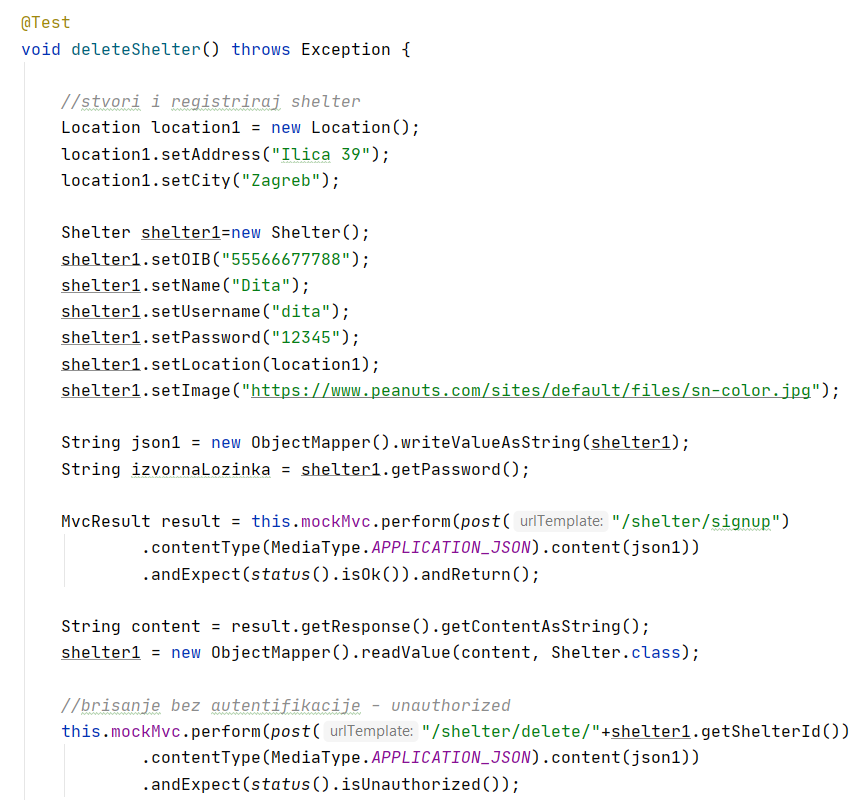
\includegraphics[scale=0.71]{slike/shelter4.1.PNG}
				\hspace*{-0.6in}
				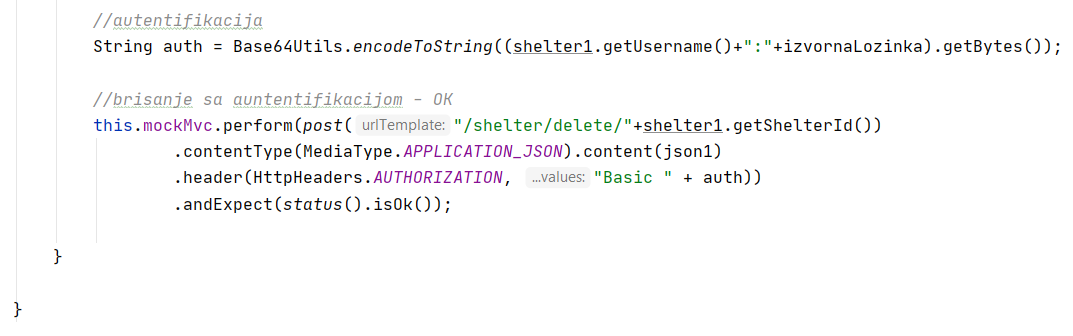
\includegraphics[scale=0.71]{slike/shelter4.2.PNG} %veličina slike u odnosu na originalnu datoteku i pozicija slike
				\centering
			\end{figure}
			
			
			
			\subsubsection{5. ispitni primjer - registracija šetača sa zauzetom email adresom}
			
			U ispitnom primjeru prvo smo stvorili dva šetača sa jednakim email adresama (ali različitim korisničkim imenima, koja također moraju biti jedinstvena). Registrirali smo prvog i dobili očekivani odgovor sa statusom 200 OK. Zatim smo pokušali registrirati drugog šetača te smo dobili  očekivani odgovor sa statusom 406 NOT ACCEPTABLE jer email adresa šetača mora biti jedinstvena.
			
			
			\begin{figure}[H]
				\centerline{
					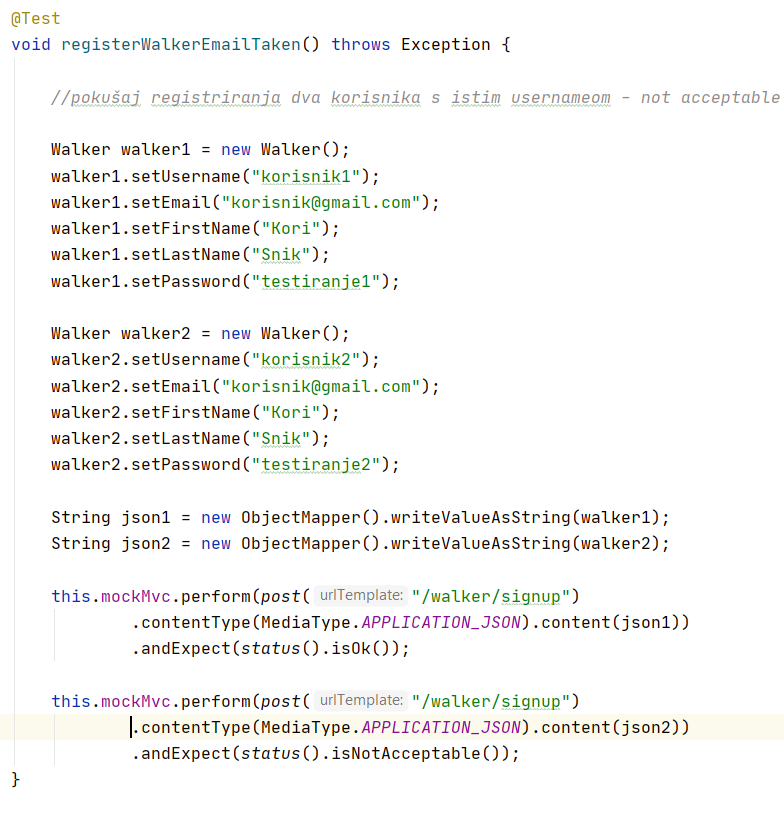
\includegraphics[scale=0.75]{slike/walker1.PNG}}
				%veličina slike u odnosu na originalnu datoteku i pozicija slike
				\centering
			\end{figure}
			
			\newpage
				
			\subsubsection{6. ispitni primjer - registracija šetača sa zauzetim korisničkim imenom}
			
			U ispitnom primjeru prvo smo stvorili dva šetača sa jednakim korisničkim imenom (ali različitim email adresama, koje također moraju biti jedinstvene). Registrirali smo prvog i dobili očekivani odgovor sa statusom 200 OK. Zatim smo pokušali registrirati drugog šetača te smo dobili  očekivani odgovor sa statusom 409 CONFLICT jer e korisničko ime šetača mora biti jedinstveno. Kao i u primjeru s udrugama, šaljemo različite statuse ovisno je li došlo do pogreške zbog korisničkog imena ili lozinke jer tako znamo kakvu poruku poslati korisniku.
			
			
			\begin{figure}[H]
				\centerline{
					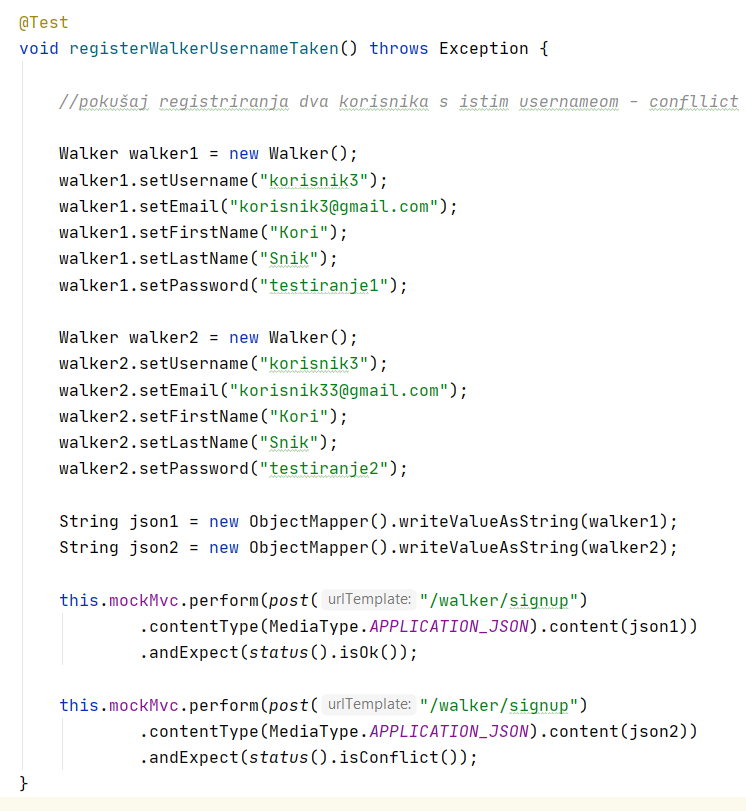
\includegraphics[scale=0.75]{slike/walker2.PNG}} %veličina slike u odnosu na originalnu datoteku i pozicija slike
				\centering
			\end{figure}
			
			
			\subsubsection{7. ispitni primjer - mijenjanje podataka šetača sa i bez autorizacije }
			
			U ispitnom primjeru prvo smo stvorili i registrirali  šetača. Dobili smo očekivani odgovor sa statusom 200 OK. Također, u tijelu odgovora nam je vraćen taj šetač kojeg smo upravo registrirali uz dodatak ID-a šetača koji je stvoren na backendu. Taj vraćeni objekt smo spremili u našu varijablu šetača jer ćemo koristiti vraćeni ID u putanji za mijenjanje podataka. Zatim smo promijenili korisničko ime šetača u "noviKorisnik" te poslali zahtjev za promjenom. Dobili smo očekivani odgovor sa statusom 401 UNAUTHORIZED jer nismo dodali autorizaciju na zahtjev. Nakon toga smo pokušali ponovno sa dodanom autorizacijom te dobili očekivani odgovor 200 OK te šetača sa promijenjenim korisničkim imenom u tijelu odgovora. Na kraju smo provjerili da je vraćenom šetaču stvarno promijenjeno ime.
			
			
			
			\begin{figure}[H]
				\hspace*{-0.58in}
				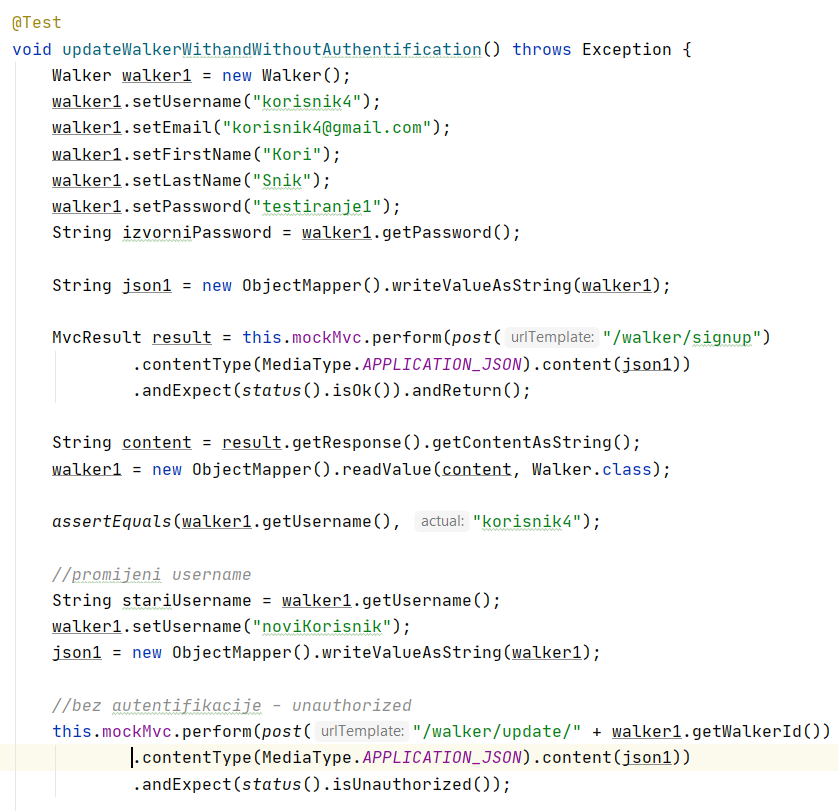
\includegraphics[scale=0.73]{slike/walker3.1.PNG}
				\hspace*{-0.41in}
				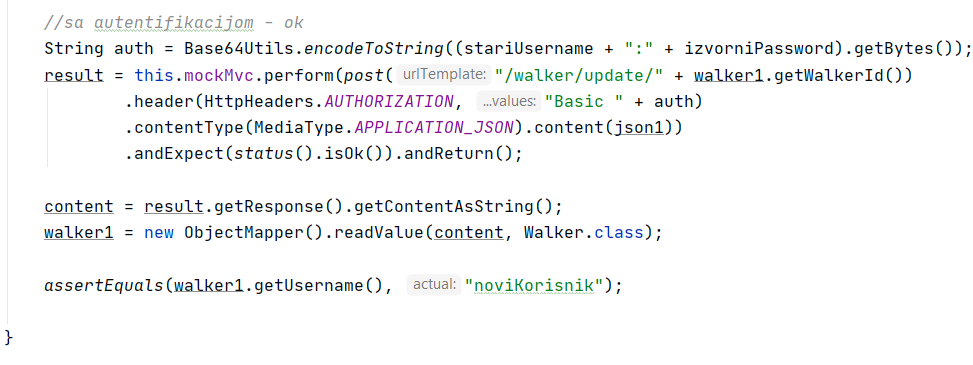
\includegraphics[scale=0.73]{slike/walker3.2.PNG} %veličina slike u odnosu na originalnu datoteku i pozicija slike
				\centering
			\end{figure}
			
			
			\subsubsection{8. ispitni primjer - mijenjanje podataka šetača sa i bez autorizacije }
			
			U ispitnom primjeru prvo smo stvorili i registrirali  šetača. Dobili smo očekivani odgovor sa statusom 200 OK.  Zatim smo stvorili novu šetnju te poslali zahtjev za rezervacijom šetnje (odabrali smo psa sa ID-jem 13 i stavili 13 u stazu "/reserve/13"). Dobili smo očekivani odgovor sa statusom 401 UNAUTHORIZED jer nismo dodali autorizaciju na zahtjev. Nakon toga smo pokušali ponovno sa dodanom autorizacijom te dobili očekivani odgovor 200 OK. 
			
			
			\begin{figure}[H]
				\hspace*{-0.18in}
				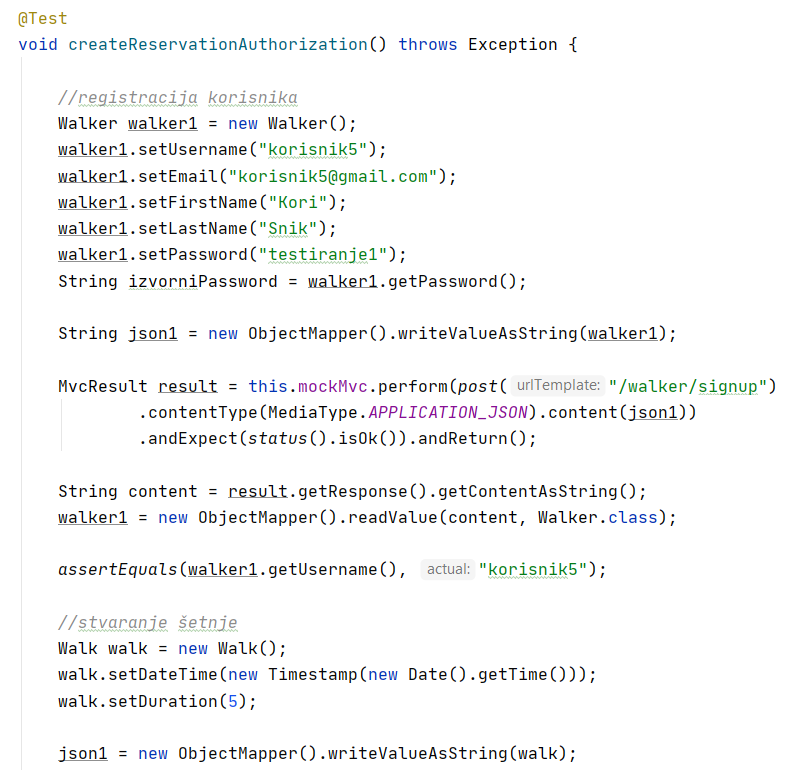
\includegraphics[scale=0.75]{slike/walker4.1.PNG}
				\hspace*{-0.4in}
				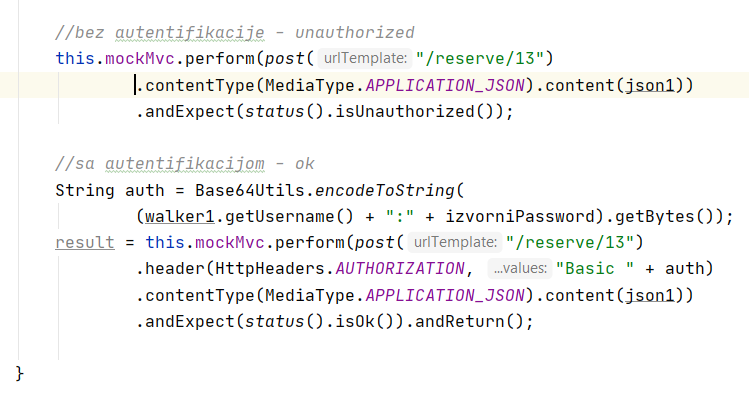
\includegraphics[scale=0.75]{slike/walker4.2.PNG} %veličina slike u odnosu na originalnu datoteku i pozicija slike
				\centering
			\end{figure}
		
		
			\subsubsection{Rezultati ispitnih primjera }
			
			\begin{figure}[H]
				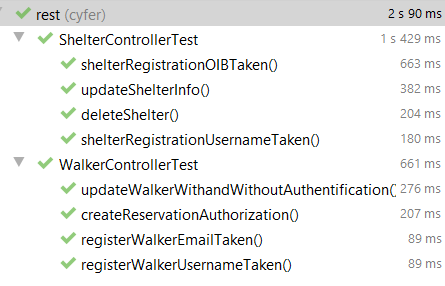
\includegraphics[scale=0.75]{slike/UnitRezultati.PNG}
				\centering
			\end{figure}
			
			
			
			
			\subsection{Ispitivanje sustava}
			
				Za ispitivanje sustava koristili smo radni okvir Selenium. Uz podršku Selenium WebDrivera, napisali smo četiri ispita u programskom jeziku Java. Kao i u gornjim primjerima, svi ispiti su uspješno prošli jer smo pri slanju krivih podataka očekivali da su korisniku prikazane informacije o tome što je krivo. Svi ispiti su vezani uz varijacije registracija šetača i udruge. Očekivali smo da sustav zna reći koji podaci su neispravni kako bi ih mogao ispraviti.
			
			\subsubsection{1. ispitni primjer - registracija šetača sa ispravnim podatcima}
			
				U ovom primjeru smo demonstrirali uspješnu registraciju šetača. Od sustava smo očekivali da nas onda preusmjeri na početnu stranicu, što je ispunjeno.
				
			 	\begin{figure}[H]
			 	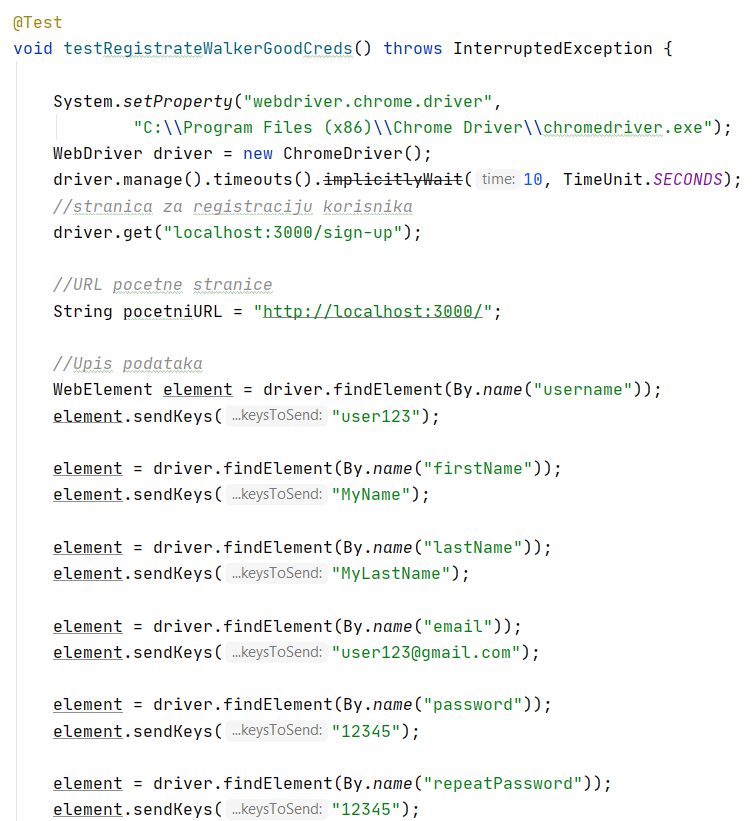
\includegraphics[scale=0.75]{slike/Selenium1.1.PNG}
			 	\hspace*{-0.85in}
			 	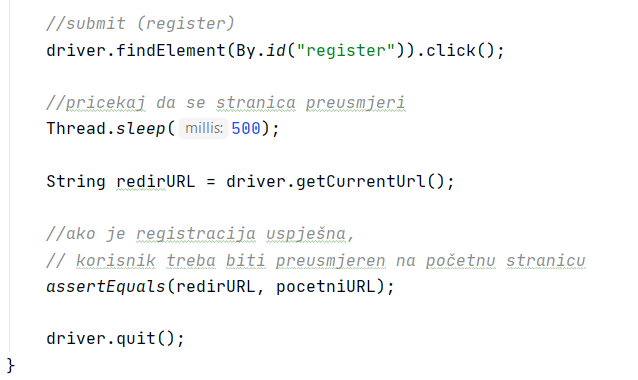
\includegraphics[scale=0.75]{slike/Selenium1.2.PNG} %veličina slike u odnosu na originalnu datoteku i pozicija slike
			 	\centering
			 \end{figure}
		 
		 
		 
		 \subsubsection{2. ispitni primjer - registracija šetača s neispravnim podatcima}
		 
		 U ovom primjeru smo demonstrirali neuspješnu registraciju šetača. Upisali smo isto korisničko ime kao i u gornjem primjeru - "user123", a kako smo ispite pokretali slijedno, takav korisnik je već bio u bazi. Od sustava smo očekivali da nam javi kakva je pogreška u pitanju. Sustav je ostao na istoj stranici (nije se dogodilo preusmjeravanje kao pri uspješnoj registraciji) te nam je ispisao poruku "Neuspješna registracija - korisničko ime je zauzeto." U ispitnom primjeru smo provjerili je li doista ispisana ta poruka. Ispod je priložena slika izvođenja u browseru te kod ispitnog primjera. 
		 
		 	\begin{figure}[H]
		 		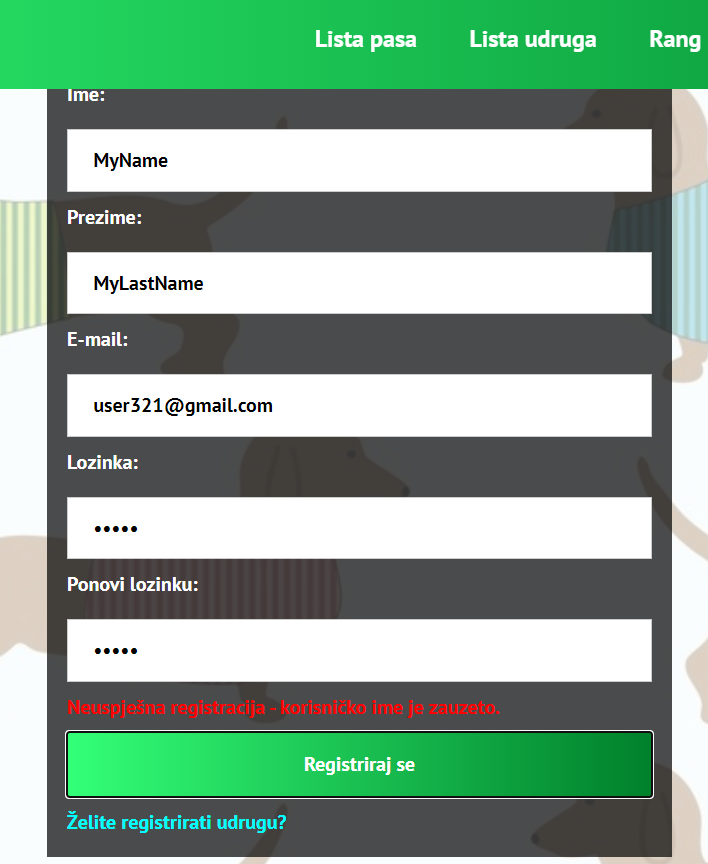
\includegraphics[scale=0.70]{slike/UsernameError.PNG}
		 		 %veličina slike u odnosu na originalnu datoteku i pozicija slike
		 		\centering
		 	\end{figure}
			 
			 \begin{figure}[H]
			 	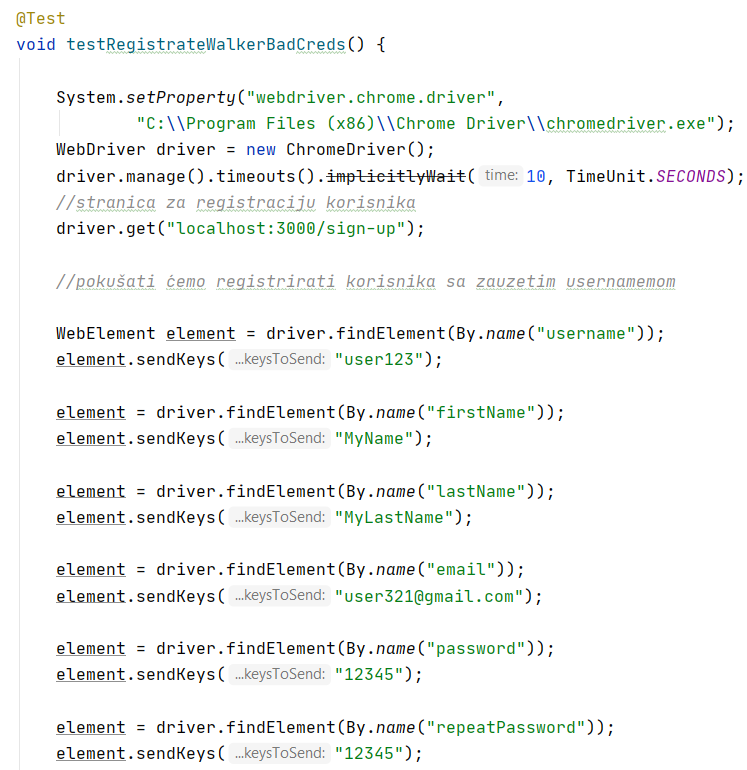
\includegraphics[scale=0.75]{slike/Selenium2.1.PNG}
			 	\hspace*{0.15in}
			 	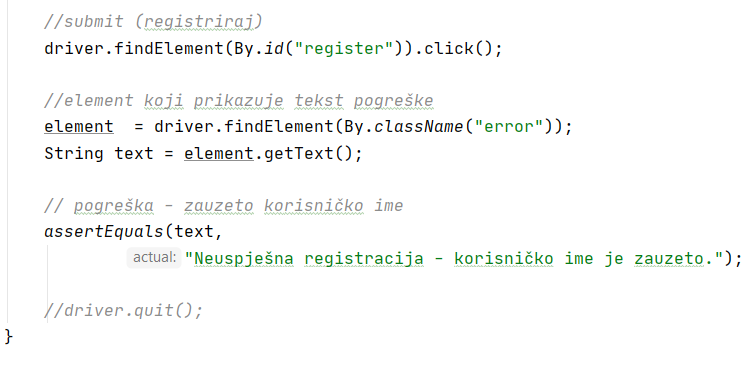
\includegraphics[scale=0.75]{slike/Selenium2.2.PNG} %veličina slike u odnosu na originalnu datoteku i pozicija slike
			 	\centering
			 \end{figure}
		 
		 
		   \subsubsection{3. ispitni primjer - registracija udruge sa ispravnim podatcima}
		 
		 U ovom primjeru smo demonstrirali uspješnu registraciju udruge uz ispravak lozinke. Upisali smo sve ispravne podatke osim lozinke i ponovljene lozinke, koje su bile različite. Od sustava smo očekivali da nam javi kakva je pogreška u pitanju. Sustav je ostao na istoj stranici (nije se dogodilo preusmjeravanje kao pri uspješnoj registraciji) te nam je ispisao poruku "Lozinke se ne poklapaju." Zatim smo ispravili ponovljenu lozinku i ponovno poslali zahtjev za registracijom. Sustav nas je očekivano preusmjerio na početnu stranicu. Ispod je priložena slika izvođenja u browseru (neispravne lozinke) te kod ispitnog primjera. 
			 
			  \begin{figure}[H]
			 	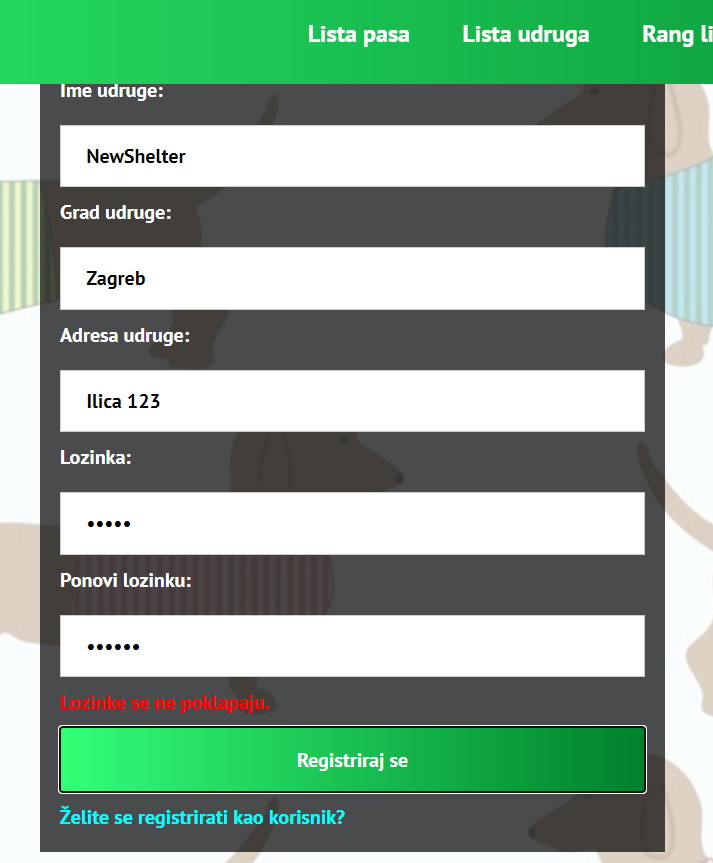
\includegraphics[scale=0.75]{slike/PasswordError.PNG}
			 	%veličina slike u odnosu na originalnu datoteku i pozicija slike
			 	\centering
			 \end{figure}
			 \begin{figure}[H]
			 	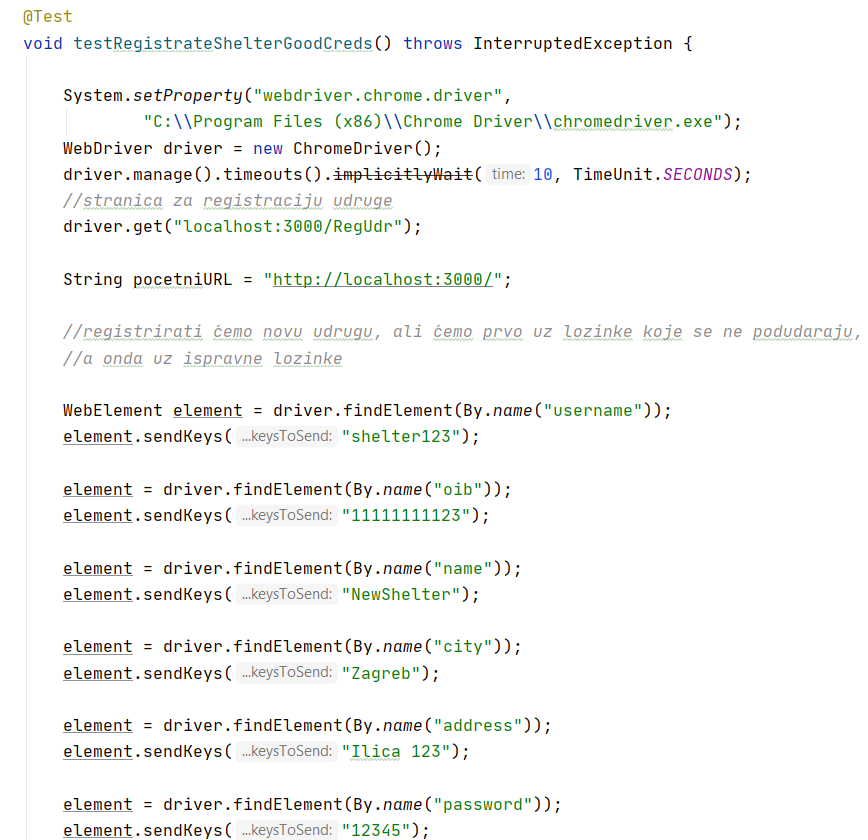
\includegraphics[scale=0.75]{slike/Selenium3.1.PNG}
			 	%veličina slike u odnosu na originalnu datoteku i pozicija slike
			 	\centering
			 \end{figure}
			 \begin{figure}[H]
			 	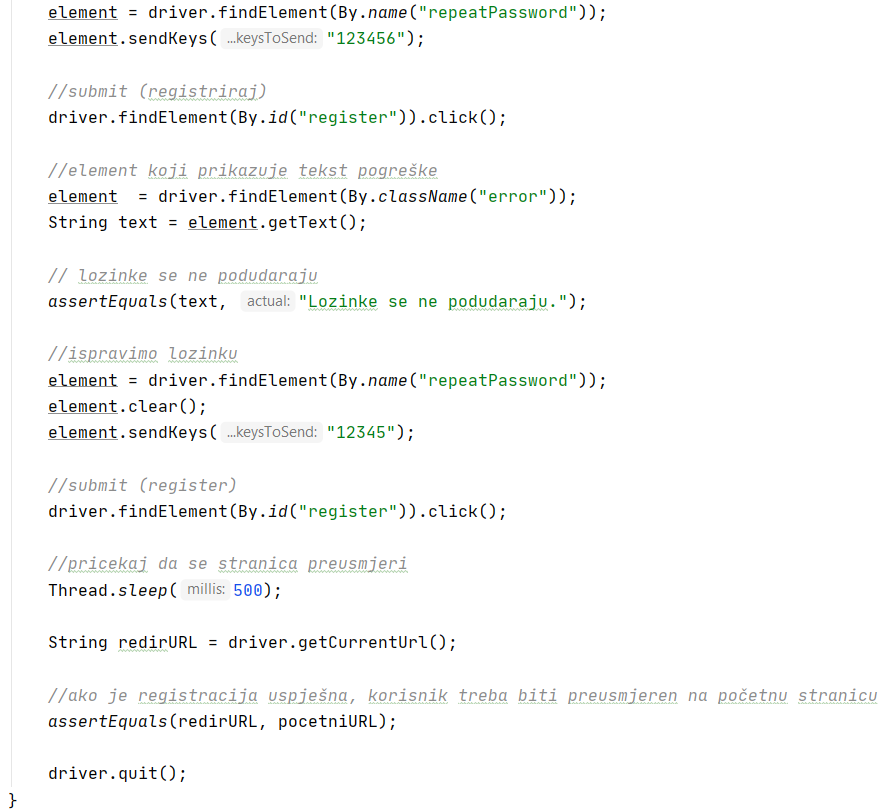
\includegraphics[scale=0.75]{slike/Selenium3.2.PNG} %veličina slike u odnosu na originalnu datoteku i pozicija slike
			 	\centering
			 \end{figure}
			 
			 
			 
			  \subsubsection{4. ispitni primjer - registracija udruge s neispravnim podatcima}
			 
			 U ovom primjeru smo demonstrirali neuspješnu registraciju udruge. Upisali smo isti OIB kao i u gornjem (trećem) primjeru - "11111111123", a kako smo ispite pokretali slijedno, takva udruga je već bila u bazi. Od sustava smo očekivali da nam javi kakva je pogreška u pitanju. Sustav je ostao na istoj stranici (nije se dogodilo preusmjeravanje kao pri uspješnoj registraciji) te nam je ispisao poruku "Neuspješna registracija - postoji već udruga sa danim OIB-om." U ispitnom primjeru smo provjerili je li doista ispisana ta poruka. Ispod je priložena slika izvođenja u browseru te kod ispitnog primjera. 
			 
			 \begin{figure}[H]
			 	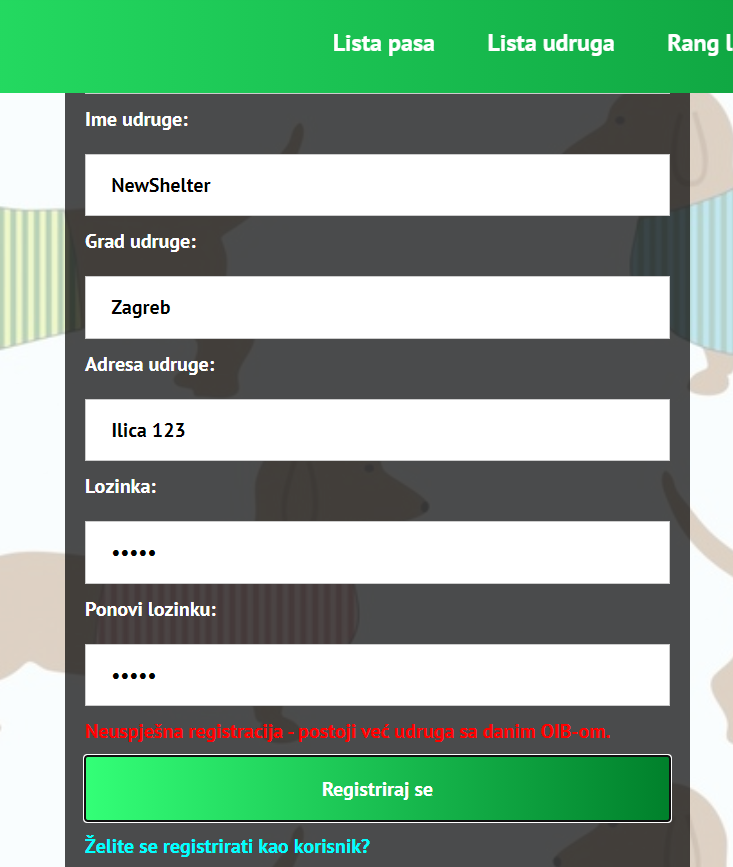
\includegraphics[scale=0.70]{slike/OIBError.PNG}
			 	%veličina slike u odnosu na originalnu datoteku i pozicija slike
			 	\centering
			 \end{figure}
			 \begin{figure}[H]
			 	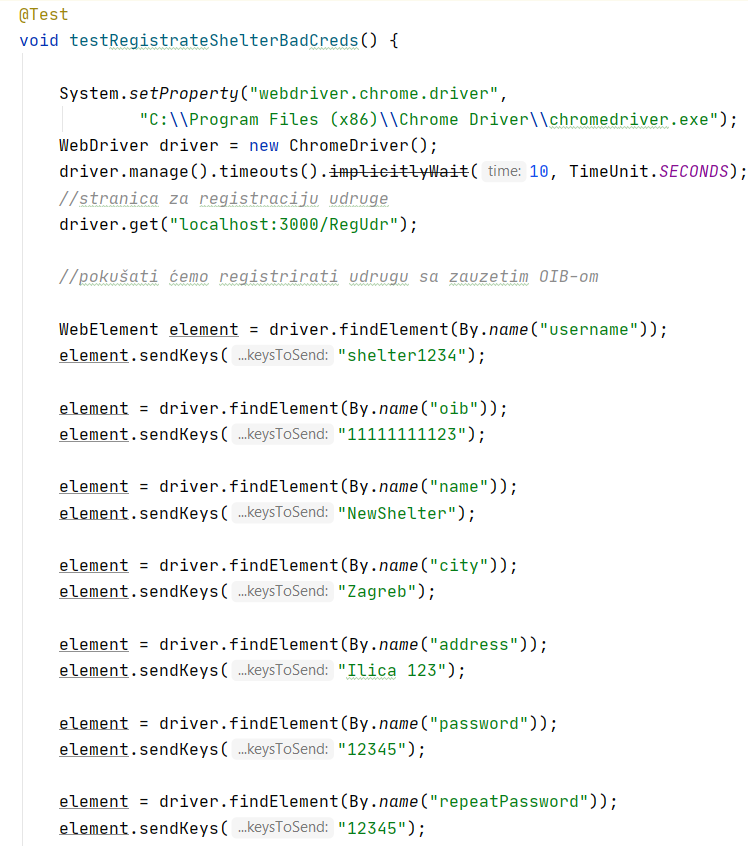
\includegraphics[scale=0.75]{slike/Selenium4.1.PNG}
			 	\hspace*{0.1in}
			 	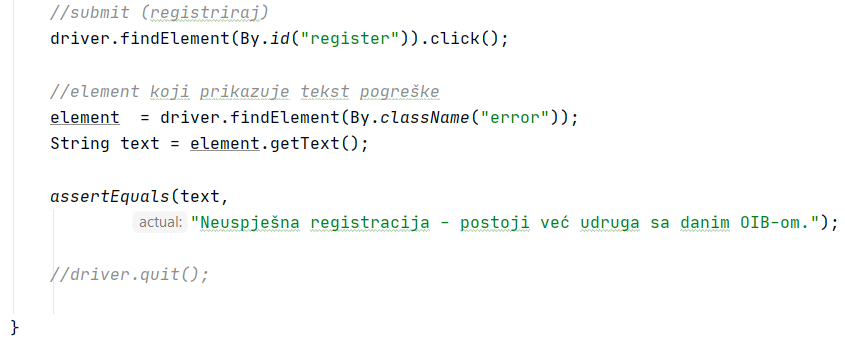
\includegraphics[scale=0.75]{slike/Selenium4.2.PNG} %veličina slike u odnosu na originalnu datoteku i pozicija slike
			 	\centering
			 \end{figure}
		 
		 
		 	\begin{figure}[H]
		 		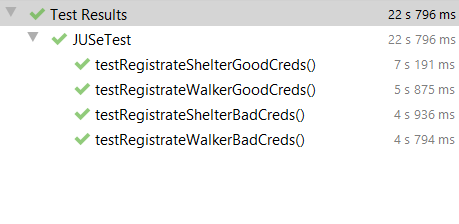
\includegraphics[scale=0.75]{slike/SeleniumRezultati.PNG} %veličina slike u odnosu na originalnu datoteku i pozicija slike
		 		\centering
		 	\end{figure}
		 
		 
			
			\eject 
		
		
		\section{Dijagram razmještaja}
			
			%\textbf{\textit{dio 2. revizije}}
			
			% \textit{Potrebno je umetnuti \textbf{specifikacijski} dijagram razmještaja i opisati ga. Moguće je umjesto specifikacijskog dijagrama razmještaja umetnuti dijagram razmještaja instanci, pod uvjetom da taj dijagram bolje opisuje neki važniji dio sustava.}
			
			\text Topologija našeg projekta sastoji se od dva čvora, od kojih su oba uređaji. Jedan je korisničko računalo, drugi je poslužiteljsko računalo. Na poslužiteljskom računalu nalaze se svi potrebni izvorni kodovi i baza podataka kako bi se ostvario uspješan deploy web aplikacije. Programska potpora sastoji se od kombinacije Spring frameworka i ReactJs-a. Također, korisničko i poslužiteljsko računalo međusobno razmjenjuju informacije putem HTTP protokola.
			
			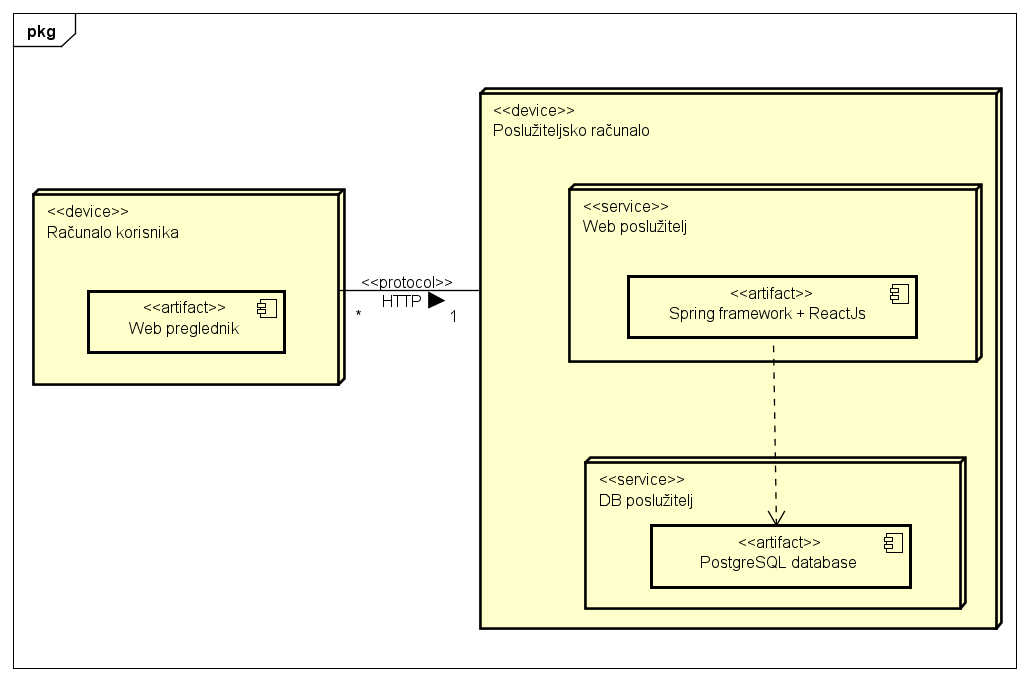
\includegraphics[scale=0.5]{dijagrami/Dijagram razmjestaja.png}
			
			\eject 
		
		\section{Upute za puštanje u pogon}
		
			\textbf{\textit{dio 2. revizije}}\\
		
			 \textit{U ovom poglavlju potrebno je dati upute za puštanje u pogon (engl. deployment) ostvarene aplikacije. Na primjer, za web aplikacije, opisati postupak kojim se od izvornog kôda dolazi do potpuno postavljene baze podataka i poslužitelja koji odgovara na upite korisnika. Za mobilnu aplikaciju, postupak kojim se aplikacija izgradi, te postavi na neku od trgovina. Za stolnu (engl. desktop) aplikaciju, postupak kojim se aplikacija instalira na računalo. Ukoliko mobilne i stolne aplikacije komuniciraju s poslužiteljem i/ili bazom podataka, opisati i postupak njihovog postavljanja. Pri izradi uputa preporučuje se \textbf{naglasiti korake instalacije uporabom natuknica} te koristiti što je više moguće \textbf{slike ekrana} (engl. screenshots) kako bi upute bile jasne i jednostavne za slijediti.}
			
			
			 \textit{Dovršenu aplikaciju potrebno je pokrenuti na javno dostupnom poslužitelju. Studentima se preporuča korištenje neke od sljedećih besplatnih usluga: \href{https://aws.amazon.com/}{Amazon AWS}, \href{https://azure.microsoft.com/en-us/}{Microsoft Azure} ili \href{https://www.heroku.com/}{Heroku}. Mobilne aplikacije trebaju biti objavljene na F-Droid, Google Play ili Amazon App trgovini.}
			
			
			\eject 